\documentclass[11pt,a4paper]{article}

\usepackage{filecontents}
\begin{filecontents*}{\jobname.bib}
  @misc{vodozemac,
    author = {{Matrix.org}},
    title = {{vodozemac: a Rust implementation of Olm and Megolm}},
    year = {2024},
    howpublished = {\url{https://github.com/matrix-org/vodozemac}},
    note = {Accessed 9 June 2026}
  }
  @misc{olmspec,
    author = {{Matrix.org}},
    title = {{The Olm Cryptographic Ratchet}},
    year = {2024},
    howpublished = {\url{https://gitlab.matrix.org/matrix-org/olm/-/blob/master/docs/olm.md}},
    note = {Accessed 9 June 2026}
  }
  @misc{megolmspec,
    author = {{Matrix.org}},
    title = {{The Megolm Group Ratchet}},
    year = {2024},
    howpublished = {\url{https://gitlab.matrix.org/matrix-org/olm/-/blob/master/docs/megolm.md}},
    note = {Accessed 9 June 2026}
  }
  @misc{zenoh-firesong,
    author = {{Eclipse Zenoh}},
    title = {{Zenoh 1.0.0 ``Firesong'' is ready to rock!}},
    howpublished = {\url{https://zenoh.io/blog/2024-10-21-zenoh-firesong/}},
    year = {2024},
    note = {Accessed 9 June 2026}
  }
  @misc{stepca,
    author = {{Smallstep}},
    title = {{step-ca: a private certificate authority}},
    year = {2024},
    howpublished = {\url{https://smallstep.com/docs/step-ca/}},
    note = {Accessed 9 June 2026}
  }
\end{filecontents*}

\usepackage[margin=2.5cm]{geometry}
\usepackage{fontspec}
\setmainfont{Latin Modern Roman}
\setsansfont{Latin Modern Sans}
\setmonofont{Hack}[Scale=0.85]
\usepackage{amssymb}
\usepackage{amsmath}
\usepackage{graphicx}
\usepackage[dvipsnames,table]{xcolor}
\usepackage{tikz}
\usetikzlibrary{positioning,arrows.meta,fit,backgrounds,shapes.geometric,calc,decorations.pathmorphing}
\usepackage{listings}
\usepackage{enumitem}
\usepackage{hyperref}
\usepackage{fancyhdr}
\usepackage{titlesec}
\usepackage{parskip}
\usepackage{float}
\usepackage{booktabs}
\usepackage{array}
\usepackage{adjustbox}
\usepackage[numbers,square,sort&compress]{natbib}
\usepackage[most]{tcolorbox}

% Colors (mirroring the sibling Zenoh security doc)
\definecolor{router}{HTML}{E74C3C}
\definecolor{peer}{HTML}{3498DB}
\definecolor{client}{HTML}{2ECC71}
\definecolor{admitted}{HTML}{2ECC71}
\definecolor{denied}{HTML}{E74C3C}
\definecolor{tls}{HTML}{2ECC71}
\definecolor{ca}{HTML}{F39C12}
\definecolor{cert}{HTML}{3498DB}
\definecolor{agent}{HTML}{3498DB}
\definecolor{machine}{HTML}{ECF0F1}
\definecolor{cipher}{HTML}{9B59B6}
\definecolor{session}{HTML}{3498DB}
\definecolor{codebg}{HTML}{F8F8F8}
\definecolor{codeframe}{HTML}{DDDDDD}
\definecolor{nixblue}{HTML}{5277C3}
\definecolor{soft}{HTML}{F4F6F8}

% Abstract box
\newtcolorbox{abstractbox}[1][]{
  enhanced, colback=soft, colframe=nixblue,
  boxrule=0.6pt, arc=2pt, left=10pt, right=10pt, top=8pt, bottom=8pt,
  title=\textbf{Abstract}, coltitle=white, colbacktitle=nixblue,
  fonttitle=\sffamily\bfseries, #1
}

% Listings style
\lstset{
  basicstyle=\ttfamily\small,
  backgroundcolor=\color{codebg},
  frame=single,
  rulecolor=\color{codeframe},
  breaklines=true,
  breakatwhitespace=true,
  tabsize=2,
  showstringspaces=false,
  keywordstyle=\color{blue},
  stringstyle=\color{red!70!black},
  commentstyle=\color{green!50!black},
}

\pagestyle{fancy}
\fancyhf{}
\fancyhead[L]{\small\textit{DVerse framework architecture}}
\fancyhead[R]{\small\textit{DVerse Platform}}
\fancyfoot[C]{\thepage}
\renewcommand{\headrulewidth}{0.4pt}

\hypersetup{
  colorlinks=true,
  linkcolor=blue!60!black,
  urlcolor=blue!60!black,
  citecolor=blue!60!black,
}

\title{%
  \vspace{-1cm}
  {\LARGE\bfseries Framework Architecture and Integration:\\
  The \texttt{bot\_framework} Crate in the DVerse Platform}
}
\author{Yordan Mitev}
\date{\today}

\begin{document}
\maketitle
\thispagestyle{fancy}

\begin{abstractbox}
  The \texttt{bot\_framework} Rust crate is the composition point
  for the DVerse platform's communication layer. The Zenoh
  router, the Tauri desktop launcher, and every demo agent in the
  repository link against it. The crate consolidates the
  decisions about certificates, mTLS, session lifecycle,
  admission, and payload encryption that are taken once and then
  reused. This document describes the crate independently of any
  one consumer, and then walks through how the router, the
  launcher, and the demo agents compose against it. It accompanies
  the sibling \emph{Zenoh evaluation and security architecture}
  document, which motivates the security model; the present
  document identifies the code that implements it.
\end{abstractbox}

\vspace{1em}

\begin{table}[H]
  \centering
  \small
  \begin{tabular}{|l|l|p{7.5cm}|}
    \hline
    \rowcolor{gray!15}
    \textbf{Version} & \textbf{Date} & \textbf{Changes} \\
    \hline
    V2 & 10 June 2026 & Rewrote prose in a formal register,
    added lists of figures, tables, and listings, and added a
    glossary. \\
    \hline
    V1 & 9 June 2026 & Initial writeup of the
    \texttt{bot\_framework} crate, with module-by-module
    descriptions and diagrams for the crate layout, module
    dependencies, router lifecycle, encrypted ping-pong, the
    \texttt{PayloadCipher} internals, and the launcher state
    machine. \\
    \hline
  \end{tabular}
  \caption{Revision history.}
  \label{tab:framework-history}
\end{table}

\newpage
\tableofcontents
\newpage
\listoffigures
\vspace{1em}
\listoftables
\vspace{1em}
\renewcommand{\lstlistlistingname}{List of Listings}
\lstlistoflistings

\newpage
% ==============================================================
\section{Introduction}
% ==============================================================

The DVerse repository is a Rust workspace. Four crates depend on a
fifth: \texttt{src/zenoh\_router/} is the per-operator router daemon,
\texttt{src/zenoh\_client\_launcher/src-tauri/} is the desktop
launcher's Rust backend, and \texttt{src/ping/} and \texttt{src/pong/}
are demo agents. All four link against \texttt{src/bot\_framework/},
which is the subject of this document.

The framework provides the components that every consumer
requires and that benefit from a single shared implementation:
certificate enrolment against step-ca, mTLS-wrapped Zenoh
sessions, agent heartbeat announcements, the wire format of the
admission handshake, the cryptographic identity binding that ties
an agent's encryption key to its TLS certificate, and the
per-process Megolm payload cipher. The router, the launcher, and
the agents combine these primitives according to their role.
Every other source file in the repository can be read as a layer
on top of the framework.

The companion document \emph{Zenoh evaluation and security
architecture} explains the security model across V1 (plain
pub/sub), V2 (mTLS), and V3 (admission and Megolm), and motivates
each layer. The present document does not repeat those arguments;
it describes the code that implements them and identifies the
entry point in the framework that each consumer calls.

\subsection{Scope}

This document covers the \texttt{bot\_framework} crate and the
parts of its three consumers that interact with the framework
directly. It does not cover the Tauri React frontend except where
the frontend illustrates the use of a framework consumer; it does
not cover the live agent-graph view in the launcher; and it does
not cover application-level agent logic. The architecture
diagrams in \texttt{documents/diagrams/} of the DVerse repository
are referenced where they apply.

% ==============================================================
\section{Crate Layout}
% ==============================================================

The \texttt{src/bot\_framework/src/} directory contains eight
modules. Each module has a single responsibility, and the public
surface is small enough that consumers can use only the modules
they need without inheriting unrelated dependencies.
Figure~\ref{fig:framework-tree} shows the layout.

\begin{figure}[H]
\centering
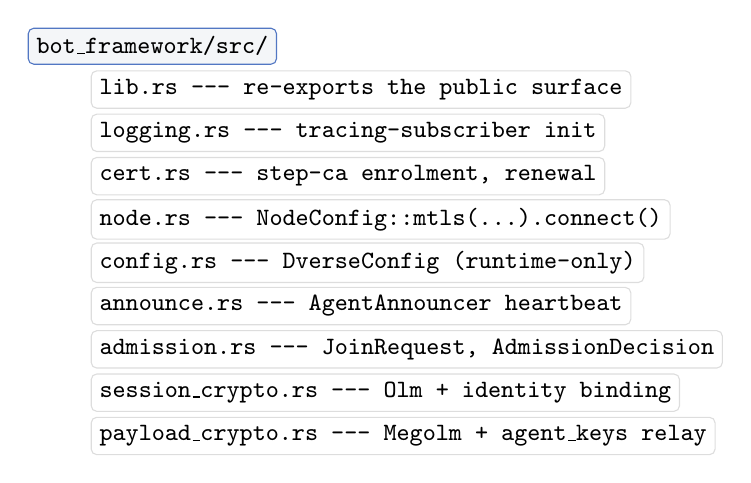
\begin{tikzpicture}[
  every node/.style={font=\ttfamily\small, inner sep=3pt, anchor=west},
  filebox/.style={draw=codeframe, rounded corners=2pt, fill=white},
  dirbox/.style={draw=nixblue, rounded corners=2pt, fill=soft, font=\ttfamily\small\bfseries},
  x=1cm, y=-0.55cm
]
  \node[dirbox]  at (0,    0) {bot\_framework/src/};
  \node[filebox] at (0.8,  1) {lib.rs --- re-exports the public surface};
  \node[filebox] at (0.8,  2) {logging.rs --- tracing-subscriber init};
  \node[filebox] at (0.8,  3) {cert.rs --- step-ca enrolment, renewal};
  \node[filebox] at (0.8,  4) {node.rs --- NodeConfig::mtls(...).connect()};
  \node[filebox] at (0.8,  5) {config.rs --- DverseConfig (runtime-only)};
  \node[filebox] at (0.8,  6) {announce.rs --- AgentAnnouncer heartbeat};
  \node[filebox] at (0.8,  7) {admission.rs --- JoinRequest, AdmissionDecision};
  \node[filebox] at (0.8,  8) {session\_crypto.rs --- Olm + identity binding};
  \node[filebox] at (0.8,  9) {payload\_crypto.rs --- Megolm + agent\_keys relay};
\end{tikzpicture}
\caption{Layout of the \texttt{bot\_framework} crate.}
\label{fig:framework-tree}
\end{figure}

\subsection{cert.rs}

This module handles step-ca~\citep{stepca} enrolment over OIDC.
The public surface is small: \texttt{cert\_path},
\texttt{key\_path}, \texttt{ca\_path}, \texttt{needs\_renewal},
and \texttt{acquire}. A consumer calls \texttt{needs\_renewal} to
determine whether a fresh certificate is required and, if so,
calls \texttt{acquire} to obtain one. The renewal threshold is
configurable; the demo agents use 23 hours, so a 24-hour leaf
certificate is rotated once per day. The on-disk layout is fixed:
each node's certificate, key, and CA bundle are stored under
\path{<cert_dir>/<node_name>/}, and the Megolm session-key files
are kept in a sibling \texttt{megolm/} directory. This co-locates
the trust material for one operator on disk.

\subsection{node.rs}

A Zenoh session is opened in the codebase only through
\texttt{NodeConfig::mtls(endpoint, ca, cert, key)} followed by
\texttt{.with\_namespace(...)} and \texttt{.connect()}. All mTLS
options (cipher suites, name-verification behaviour, listener
versus connector role) are encapsulated by the builder.
Centralising these options localises the security policy:
changing how the platform trusts a peer requires editing one file.
The builder pattern also keeps call sites readable; an agent's
main function does not need to be aware that Zenoh accepts a JSON5
configuration blob.

\subsection{config.rs}

\texttt{DverseConfig} holds the operator's runtime state: the
router endpoint, the certificate directory, the session role
(admin or client), the session identifier, and OIDC credentials.
The configuration is runtime-only, by design. Restarting the
launcher returns the operator to the login screen rather than
rejoining the last session automatically. Joining a session is a
security-relevant action and is required to be explicit on every
launch.

\subsection{announce.rs}

\texttt{AgentAnnouncer::start(session, AgentInfo \{ ... \})}
returns a handle that publishes a heartbeat at a fixed cadence
and stops publishing when dropped. The router consumes these
heartbeats to drive the live agent graph in the launcher.
Dropping the handle is the cleanup signal: the router observes
the gap, marks the agent \texttt{Degraded}, then \texttt{Offline},
and finally evicts it from its known-agents map.

\subsection{admission.rs}

This module defines two JSON-serialisable wire structures:
\texttt{JoinRequest} and \texttt{AdmissionDecision \{ Allow, Deny
\}}. The handshake itself is implemented in the router crate
(\texttt{admission\_handler.rs}), which reads the requester's CN
from its mTLS connection, verifies the binding signature, and
either wraps the Megolm \texttt{SessionKey} in an Olm pre-key
message or publishes a \texttt{Deny} with a reason field. The
wire format is defined in the framework because both sides of the
handshake must agree on it: one side runs in the router, the
other in any node that requests to join.

\subsection{session\_crypto.rs}

This module has two responsibilities. The first is the
cryptographic identity binding that demonstrates that a
vodozemac~\citep{vodozemac} Curve25519 identity key belongs to
the holder of the leaf certificate.
\texttt{sign\_enc\_binding\_pem} takes the operator's TLS private
key (PEM), the operator's CN, and the Curve25519 identity key,
and produces an ECDSA P-256 signature over a domain-separated,
length-prefixed message
\[
  \texttt{"dverse/enc-key-binding/v1\textbackslash 0"}
  \ \Vert\ \texttt{cn\_len}
  \ \Vert\ \texttt{cn}
  \ \Vert\ \texttt{curve25519\_key}.
\]
The verifier extracts the P-256 public key from the leaf
certificate and rejects the binding on any signature mismatch, CN
mismatch, or mismatch between the claimed CN and the CN in the
certificate.

The second responsibility is the Olm session machinery used by
the admin to wrap the Megolm \texttt{SessionKey} for a specific
requester. The admin holds one Olm identity per session; the
requester publishes a one-time prekey alongside its identity key
in its \texttt{JoinRequest}, and the admin's
\texttt{olm\_encrypt\_to} produces a pre-key message addressed to
that prekey. The Olm session created by this step is persisted in
the admin's crypto state, allowing later messages to the same
requester to be encrypted with a non-prekey Olm message if needed.

\subsection{payload\_crypto.rs}

This module implements the per-process Megolm~\citep{megolmspec}
cipher. \texttt{PayloadCipher} owns one outbound
\texttt{GroupSender} and a map of inbound
\texttt{GroupReceiver}s keyed by \texttt{session\_id}. The
public surface is small: \texttt{encrypt(bytes)},
\texttt{decrypt(bytes)} (which dispatches to the correct receiver
based on the wire envelope's \texttt{sender\_id}),
\texttt{publish\_session\_key} (writes the outbound key to disk
for same-machine peers), and \texttt{refresh\_receivers}
(re-scans the \texttt{megolm/} directory for peer key files that
have appeared since the last call).

Cross-machine key distribution is also implemented in this
module, in
\texttt{spawn\_agent\_key\_relay(cipher, session, cn, agent\_name)}.
The function spawns two background tokio tasks: an announce task
that publishes the local outbound \texttt{session\_key\_b64} on
\path{dverse/agent_keys/<cn>/<agent_name>} every five seconds,
and a subscribe task that calls \texttt{install\_peer\_session\_key}
on each received envelope. The install routine skips
self-announcements (a node never installs a receiver for its own
sender), is idempotent on re-installation of an already known
peer, and logs the installed session identifier for tracing.
Because the topic falls under the broad fabric ACL rule, only
admitted CNs receive these messages; admission is the trust
boundary for key distribution.

\paragraph{An intentional carve-out: the cipher sits beside the session, not inside it.}
In the current implementation, encryption is a layer that the
agent applies to its bytes before passing them to a Zenoh
\texttt{put}, and re-applies on the way out of a subscriber. The
Zenoh session itself is not aware of the cipher: a \texttt{put}
on \texttt{dverse/ping} succeeds whether or not the bytes were
encrypted, so an agent that omits the call to
\texttt{cipher.encrypt} would publish plaintext on the same topic
without any framework-level refusal. Encryption is therefore
enforced by convention (every agent template wraps its outbound
bytes) rather than by the API. In the current state of the
project this is best described as optional encryption that every
agent in the repository opts into.

The intended end state is the opposite: the cipher moves inside
the Zenoh session, so a session opened on the dverse fabric
carries only encrypted payloads, with no application-layer
choice. The expected shape is a wrapper around \texttt{Session::put}
and \texttt{Session::declare\_subscriber} that encrypts and
decrypts on the way through, removing the possibility of an
agent author skipping the cipher entirely. The cross-machine
\texttt{agent\_keys/**} relay would then operate inside the
session as an internal side channel rather than as a function
the agent invokes directly. After that change, an agent cannot
publish plaintext even by mistake, and the invariant of no
unencrypted communication on the dverse fabric becomes a
property of the API rather than a property of the convention.

\subsection{Who uses what}

Each consumer in the workspace depends on a different subset of
the framework's modules. Figure~\ref{fig:framework-deps} maps
the dependencies. The router uses every module except
\texttt{payload\_crypto}; the launcher uses the same set minus
\texttt{node} and \texttt{announce}; the demo agents use the
modules required to connect, announce, encrypt, and relay
session keys.

\begin{figure}[H]
\centering
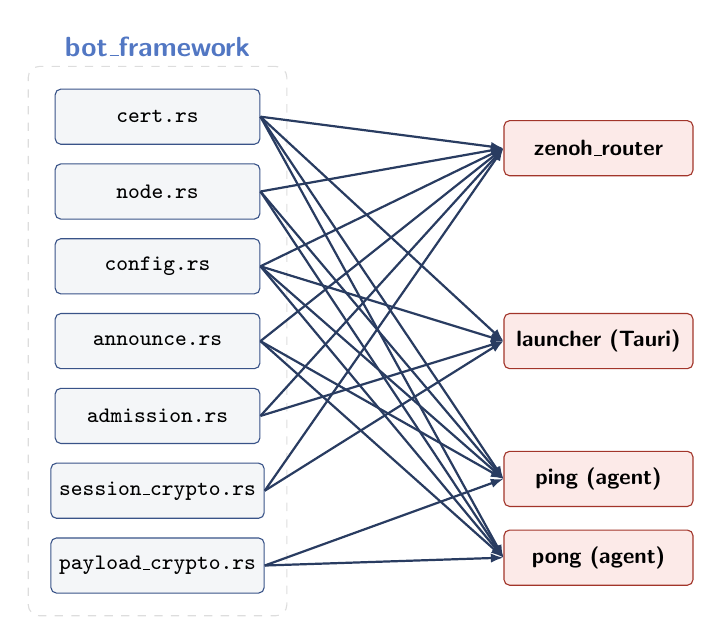
\begin{tikzpicture}[
  every node/.style={font=\sffamily\footnotesize},
  modbox/.style={
    draw=nixblue!70!black, fill=soft, rounded corners=2pt,
    minimum width=2.6cm, minimum height=0.7cm, align=center,
    inner sep=3pt, font=\ttfamily\footnotesize,
  },
  consumerbox/.style={
    draw=router!70!black, fill=router!12, rounded corners=2pt,
    minimum width=2.4cm, minimum height=0.7cm, align=center,
    inner sep=3pt, font=\sffamily\bfseries\footnotesize,
  },
  dep/.style={-{Latex[length=1.6mm]}, thick, draw=nixblue!50!black},
  groupbox/.style={
    draw=codeframe, dashed, rounded corners=4pt, inner sep=8pt,
  },
]
  \node[modbox] (mcert)     at (0,    0)    {cert.rs};
  \node[modbox] (mnode)     at (0,   -0.95) {node.rs};
  \node[modbox] (mcfg)      at (0,   -1.9)  {config.rs};
  \node[modbox] (mann)      at (0,   -2.85) {announce.rs};
  \node[modbox] (madm)      at (0,   -3.8)  {admission.rs};
  \node[modbox] (mscry)     at (0,   -4.75) {session\_crypto.rs};
  \node[modbox] (mpcry)     at (0,   -5.7)  {payload\_crypto.rs};
  \node[groupbox, fit=(mcert)(mpcry),
        label={[font=\sffamily\bfseries, text=nixblue]above:bot\_framework}] {};

  \node[consumerbox] (router)   at (5.6, -0.4)  {zenoh\_router};
  \node[consumerbox] (launcher) at (5.6, -2.85) {launcher (Tauri)};
  \node[consumerbox] (ping)     at (5.6, -4.6)  {ping (agent)};
  \node[consumerbox] (pong)     at (5.6, -5.6)  {pong (agent)};

  % router uses everything except payload_crypto
  \draw[dep] (mcert.east)   -- (router.west);
  \draw[dep] (mnode.east)   -- (router.west);
  \draw[dep] (mcfg.east)    -- (router.west);
  \draw[dep] (mann.east)    -- (router.west);
  \draw[dep] (madm.east)    -- (router.west);
  \draw[dep] (mscry.east)   -- (router.west);

  % launcher: cert (renewal trigger), config (DverseConfig), admission
  % (allow/deny commands), session_crypto (to inspect crypto state for UI)
  \draw[dep] (mcert.east)   -- (launcher.west);
  \draw[dep] (mcfg.east)    -- (launcher.west);
  \draw[dep] (madm.east)    -- (launcher.west);
  \draw[dep] (mscry.east)   -- (launcher.west);

  % agents: cert, node, config, announce, payload_crypto
  \draw[dep] (mcert.east)   -- (ping.west);
  \draw[dep] (mnode.east)   -- (ping.west);
  \draw[dep] (mcfg.east)    -- (ping.west);
  \draw[dep] (mann.east)    -- (ping.west);
  \draw[dep] (mpcry.east)   -- (ping.west);
  \draw[dep] (mcert.east)   -- (pong.west);
  \draw[dep] (mnode.east)   -- (pong.west);
  \draw[dep] (mcfg.east)    -- (pong.west);
  \draw[dep] (mann.east)    -- (pong.west);
  \draw[dep] (mpcry.east)   -- (pong.west);
\end{tikzpicture}
\caption{Module dependencies of the framework's consumers.}
\label{fig:framework-deps}
\end{figure}

The asymmetry between the agents' and the router's dependency
sets is deliberate. The agents do not import
\texttt{admission.rs} because the admission handshake is run by
the operator's router, not by the agents. The router does not
import \texttt{payload\_crypto.rs} because the router routes
ciphertext without decrypting it. This separation enables the
router to carry traffic for a session whose Megolm key it does
not hold: routing and decryption are distinct concerns, and the
framework keeps them in separate modules.

% ==============================================================
\section{How the Router Uses the Framework}
\label{sec:howRouterUses}
% ==============================================================

The Zenoh router consumes the largest portion of the framework.
It requires the certificate pipeline, the mTLS Zenoh session, the
admission handshake, and the session-crypto identity primitives.
It does not require \texttt{payload\_crypto.rs}: the router does
not encrypt agent payloads; it routes them. Encryption and
decryption are performed by the agents.

\subsection{Lifecycle of one session}

Figure~\ref{fig:router-lifecycle} shows the lifecycle of a single
session in the router, from operator login to the first agent
payload.

\begin{figure}[H]
\centering
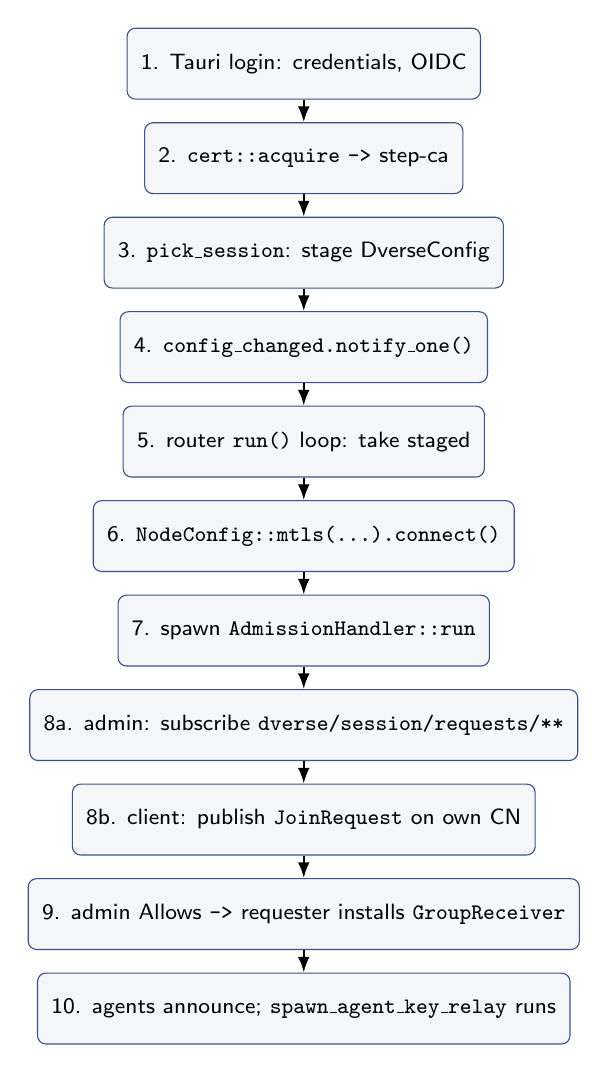
\begin{tikzpicture}[
  every node/.style={font=\sffamily\footnotesize},
  lstep/.style={
    draw=nixblue!70!black, fill=soft, rounded corners=3pt,
    minimum width=4cm, minimum height=0.9cm, align=left,
    inner sep=5pt,
  },
  arrow/.style={-{Latex[length=2mm]}, thick},
  swimlane/.style={
    draw=codeframe, fill=none, rounded corners=4pt, inner sep=8pt,
  },
  lanelabel/.style={font=\sffamily\bfseries\footnotesize, text=nixblue},
]
  \node[lstep] (s1) at (0, 0)    {1. Tauri login: credentials, OIDC};
  \node[lstep] (s2) at (0, -1.2) {2. \texttt{cert::acquire} \texttt{->} step-ca};
  \node[lstep] (s3) at (0, -2.4) {3. \texttt{pick\_session}: stage DverseConfig};
  \node[lstep] (s4) at (0, -3.6) {4. \texttt{config\_changed.notify\_one()}};
  \node[lstep] (s5) at (0, -4.8) {5. router \texttt{run()} loop: take staged};
  \node[lstep] (s6) at (0, -6.0) {6. \texttt{NodeConfig::mtls(...).connect()}};
  \node[lstep] (s7) at (0, -7.2) {7. spawn \texttt{AdmissionHandler::run}};
  \node[lstep] (s8) at (0, -8.4) {8a. admin: subscribe \texttt{dverse/session/requests/**}};
  \node[lstep] (s9) at (0, -9.6) {8b. client: publish \texttt{JoinRequest} on own CN};
  \node[lstep] (s10) at (0, -10.8) {9. admin Allows \texttt{->} requester installs \texttt{GroupReceiver}};
  \node[lstep] (s11) at (0, -12.0) {10. agents announce; \texttt{spawn\_agent\_key\_relay} runs};

  \draw[arrow] (s1) -- (s2);
  \draw[arrow] (s2) -- (s3);
  \draw[arrow] (s3) -- (s4);
  \draw[arrow] (s4) -- (s5);
  \draw[arrow] (s5) -- (s6);
  \draw[arrow] (s6) -- (s7);
  \draw[arrow] (s7) -- (s8);
  \draw[arrow] (s8) -- (s9);
  \draw[arrow] (s9) -- (s10);
  \draw[arrow] (s10) -- (s11);
\end{tikzpicture}
\caption{Lifecycle of one router session.}
\label{fig:router-lifecycle}
\end{figure}

Each step in the figure corresponds to a specific entry point in
the framework. Steps 2--6 use \texttt{cert.rs} and
\texttt{node.rs};
step 7 instantiates the router's own admission handler, which uses
\texttt{admission.rs} for the wire format and \texttt{session\_crypto.rs}
for the Olm wrap; step 11 runs the agent code, which adds the only
\texttt{payload\_crypto.rs} layer.

\subsection{Why config\_changed is a framework concern}

The framework defines \texttt{DverseConfig} and exposes the
mechanism for staging a new configuration (the router crate
consumes \texttt{config\_changed} via the state's
\texttt{Arc<Notify>}). The mechanism is located in the framework
because the same contract is required for the router and for any
other tool that drives the router, such as an integration test or
an alternative user interface. Locating the notification in the
framework makes the contract explicit: a consumer rings the
doorbell when the router should pick up a new configuration.

% ==============================================================
\section{How Agents Use the Framework}
% ==============================================================

An agent consists of approximately eighty lines of integration
code. The demo \texttt{ping} agent is shown in
Listing~\ref{lst:ping}; \texttt{pong} is structurally identical,
with publish and subscribe topics swapped. The agent interacts
with the framework at four points: the certificate renewal call,
the \texttt{NodeConfig} connection, the announcer, and the
cipher together with the agent-key relay.

\begin{lstlisting}[caption={The full \texttt{ping} agent
(\texttt{src/ping/src/main.rs}).},label={lst:ping}]
const NODE_NAME: &str = "ping";

#[tokio::main]
async fn main() -> Result<()> {
    bot_framework::logging::init();
    let cfg = DverseConfig::load()
        .expect("No dverse config found. Run the router first to log in.");

    if cert::needs_renewal(&cert_path, /* 23h */, Some(&cfg.operator_cn())).await {
        cert::acquire(&cfg.cert_config_for(NODE_NAME)?).await?;
    }

    let session = NodeConfig::mtls(&cfg.router_endpoint, &ca, &cert, &key)
        .with_namespace(cfg.session_id())
        .connect()
        .await?;

    let _announcer = AgentAnnouncer::start(session.clone(), AgentInfo {
        cn: &cfg.operator_cn(),
        agent_name: NODE_NAME,
        publishes: vec!["dverse/ping".into()],
        subscribes: vec!["dverse/pong".into()],
        version: env!("CARGO_PKG_VERSION"),
    });

    let crypto_dir = cfg.cert_dir.join("megolm");
    let cipher = Arc::new(Mutex::new(PayloadCipher::new(NODE_NAME, &crypto_dir)?));
    cipher.lock().unwrap().publish_session_key(&crypto_dir, NODE_NAME)?;
    payload_crypto::spawn_agent_key_relay(
        Arc::clone(&cipher), session.clone(),
        cfg.operator_cn().to_string(), NODE_NAME.to_string(),
    );

    // Loop: refresh receivers, encrypt, publish, await pong, decrypt.
}
\end{lstlisting}

The same pattern is used by every agent. The framework keeps the
four required calls (mTLS connect, announce, cipher, relay)
concise so that the agent author can focus on application logic.
Certificate renewal is a single branch; if the cached certificate
is still within its lifetime, no enrolment work is performed.

\subsection{The \texttt{Arc<Mutex<PayloadCipher>>} pattern}

The cipher is shared across three call sites: the main loop
(\texttt{encrypt}, \texttt{decrypt}, \texttt{refresh\_receivers}),
the announce task spawned by the relay (which reads
\texttt{my\_session\_key\_b64}), and the subscribe task spawned by
the relay (which calls \texttt{install\_peer\_session\_key}).
Wrapping the cipher in \texttt{Arc<Mutex<...>>} is a direct way
to share mutable state across those tasks. The lock is held only
briefly, and no \texttt{await} is performed while the lock is
held.

\subsection{Encrypted ping-pong, end to end}

Figure~\ref{fig:ping-pong-encrypted} shows one round of encrypted
ping-pong between two operators. The agents run on separate
machines; the agent-key relay provides each operator with the
other's \texttt{GroupReceiver}.

\begin{figure}[H]
\centering
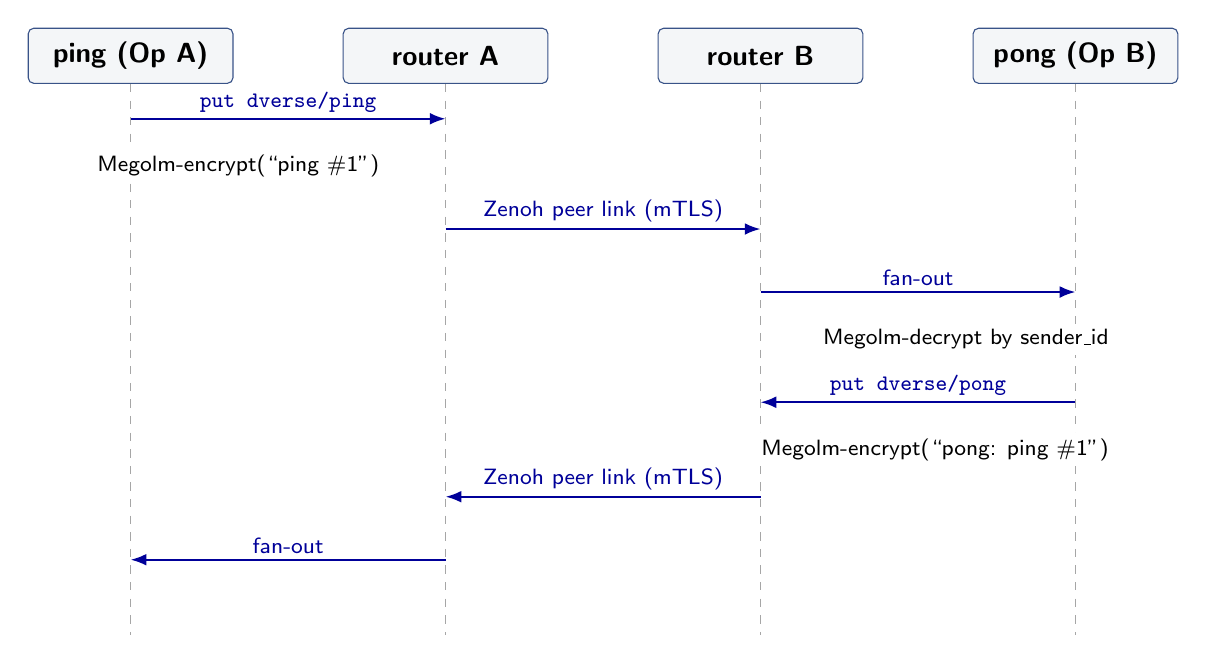
\begin{tikzpicture}[
  every node/.style={font=\sffamily\footnotesize},
  actor/.style={
    draw=nixblue!70!black, fill=soft, rounded corners=2pt,
    minimum width=2.6cm, minimum height=0.7cm,
    font=\sffamily\bfseries,
  },
  lstep/.style={
    font=\footnotesize\sffamily, fill=white, inner sep=2pt,
  },
  arrow/.style={-{Latex[length=2mm]}, thick, blue!60!black},
  life/.style={dashed, gray!70},
]
  \node[actor] (pingA) at (0, 0)  {ping (Op A)};
  \node[actor] (rA)    at (4, 0)  {router A};
  \node[actor] (rB)    at (8, 0)  {router B};
  \node[actor] (pongB) at (12, 0) {pong (Op B)};

  \draw[life] (pingA.south) -- ++(0,-7);
  \draw[life] (rA.south)    -- ++(0,-7);
  \draw[life] (rB.south)    -- ++(0,-7);
  \draw[life] (pongB.south) -- ++(0,-7);

  \draw[arrow] (pingA |- 0,-0.8) -- (rA |- 0,-0.8)
    node[lstep, midway, above] {\texttt{put dverse/ping}};
  \node[lstep, anchor=west] at (-0.5,-1.4) {Megolm-encrypt(``ping \#1'')};

  \draw[arrow] (rA |- 0,-2.2) -- (rB |- 0,-2.2)
    node[lstep, midway, above] {Zenoh peer link (mTLS)};

  \draw[arrow] (rB |- 0,-3.0) -- (pongB |- 0,-3.0)
    node[lstep, midway, above] {fan-out};
  \node[lstep, anchor=east] at (12.5,-3.6) {Megolm-decrypt by sender\_id};

  \draw[arrow] (pongB |- 0,-4.4) -- (rB |- 0,-4.4)
    node[lstep, midway, above] {\texttt{put dverse/pong}};
  \node[lstep, anchor=east] at (12.5,-5.0) {Megolm-encrypt(``pong: ping \#1'')};

  \draw[arrow] (rB |- 0,-5.6) -- (rA |- 0,-5.6)
    node[lstep, midway, above] {Zenoh peer link (mTLS)};

  \draw[arrow] (rA |- 0,-6.4) -- (pingA |- 0,-6.4)
    node[lstep, midway, above] {fan-out};
\end{tikzpicture}
\caption{One round trip of encrypted ping-pong between two
operators.}
\label{fig:ping-pong-encrypted}
\end{figure}

The figure illustrates the layering. The routers carry every
payload without the ability to read it; the operators hold the
trust, because they decide who is admitted to the session. A
compromised router exposes only routing metadata.

\subsection{Inside the PayloadCipher}

Each agent process owns one \texttt{PayloadCipher}, but the
cipher's internal structure is asymmetric: it has one outbound
\texttt{GroupSender} and a map of inbound \texttt{GroupReceiver}s
keyed by the session identifier of the peer that produced each
receiver. Figure~\ref{fig:cipher-shape} shows the cipher state
during a steady-state run of \texttt{ping} on operator A,
communicating with two other agents.

\begin{figure}[H]
\centering
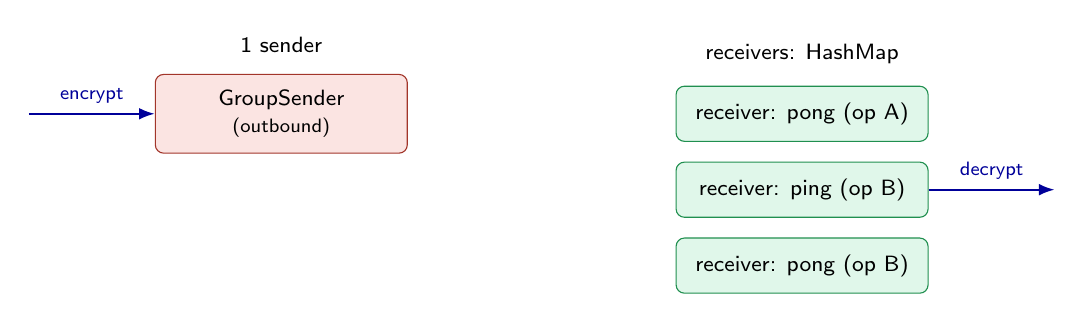
\begin{tikzpicture}[
  every node/.style={font=\sffamily\footnotesize},
  sender/.style={
    draw=router!70!black, fill=router!15, rounded corners=3pt,
    minimum width=3.2cm, minimum height=1cm, align=center,
  },
  receiver/.style={
    draw=admitted!70!black, fill=admitted!15, rounded corners=3pt,
    minimum width=3.2cm, minimum height=0.7cm, align=center,
  },
  arrow/.style={-{Latex[length=2mm]}, thick, blue!60!black},
]
  % Sender (single, on the left)
  \node[sender] (snd) {GroupSender\\\scriptsize (outbound)};
  \node[font=\footnotesize\sffamily, above=0.15cm of snd] {1 sender};

  % Receivers (stacked, on the right)
  \node[receiver, right=3.4cm of snd] (r1) {receiver: pong (op A)};
  \node[receiver, below=0.25cm of r1]  (r2) {receiver: ping (op B)};
  \node[receiver, below=0.25cm of r2]  (r3) {receiver: pong (op B)};
  \node[font=\footnotesize\sffamily, above=0.15cm of r1] {receivers: HashMap};

  % encrypt / decrypt arrows
  \draw[arrow] ($(snd.west)+(-1.6,0)$) -- node[above,font=\scriptsize\sffamily]{encrypt} (snd.west);
  \draw[arrow] (r2.east) -- node[above,font=\scriptsize\sffamily]{decrypt} ($(r2.east)+(1.6,0)$);
\end{tikzpicture}
\caption{\texttt{PayloadCipher}: one sender, N receivers keyed by
peer \texttt{session\_id}. \texttt{decrypt} dispatches by the wire
envelope's \texttt{sender\_id}.}
\label{fig:cipher-shape}
\end{figure}

The deduplication logic in
\texttt{install\_peer\_session\_key} corresponds directly to the
figure. An envelope whose session identifier matches the local
sender is discarded, because a node never installs a receiver
for its own outgoing key. An envelope whose session identifier
is already a key in the map is also discarded, making the
operation idempotent. The receiver map grows only when a new
peer is observed.

% ==============================================================
\section{How the Launcher Uses the Framework}
% ==============================================================

The desktop launcher is a Tauri 2 application. Its Rust backend
(\path{src/zenoh_client_launcher/src-tauri/}) exposes a small set
of commands to the React frontend: \texttt{login},
\texttt{pick\_session}, \texttt{admit\_request},
\texttt{deny\_request}, and \texttt{logout}. Each command is a
wrapper around one or two framework calls.

\subsection{Command surface}

\texttt{login} runs the OIDC flow through Keycloak, passes the
returned token to \texttt{cert::acquire}, and writes the resulting
certificate into the operator's certificate directory. The
function does not select a session; the operator is then
presented with the chooser screen.

\texttt{pick\_session} builds a \texttt{DverseConfig} from the
chooser's selection (a discovered admin's CN, or \texttt{None}
when the operator chooses to create a new session as admin) and
stages the configuration on the router state. The command then
calls \texttt{config\_changed.notify\_one()}. The router crate's
\texttt{run()} loop consumes the staged configuration on its next
iteration. The Tauri command returns immediately, the user
interface displays a loading screen, and the frontend polls
router state for the next transition.

\texttt{admit\_request} and \texttt{deny\_request} dispatch to
the admin's admission handler. The admit path performs the Olm
wrap of the Megolm session key for the named requester and
publishes the \texttt{Allow}; the deny path publishes a
\texttt{Deny} with a reason supplied by the admin.

\texttt{logout} drops the router's current Zenoh session, clears
the runtime \texttt{DverseConfig}, and rings
\texttt{config\_changed} so that the router halts the existing
session. The launcher returns the operator to the login screen.

\subsection{Frontend components}

Three React components implement the admission user interface.
\texttt{ChooserScreen} renders the list of admins discovered over
mDNS along with a button to create a new session and a logout
button. \texttt{RequestingJoinScreen} displays a spinner and the
admin's CN while the operator's \texttt{JoinRequest} is in
flight, and transitions either to a denial notification or to the
main screen, depending on the admission outcome.
\texttt{PendingRequestsPanel} is rendered within the admin's main
screen and lists each pending requester together with allow and
deny buttons. The components are state-driven views over router
state retrieved through the command interface; they do not hold
framework objects directly.

\subsection{Launcher state machine}

The launcher's user interface is a finite state machine driven by
router state. Figure~\ref{fig:launcher-fsm} shows the screens and
the events that cause transitions between them. Each transition
corresponds to a specific framework call on the Tauri command
surface.

\begin{figure}[H]
\centering
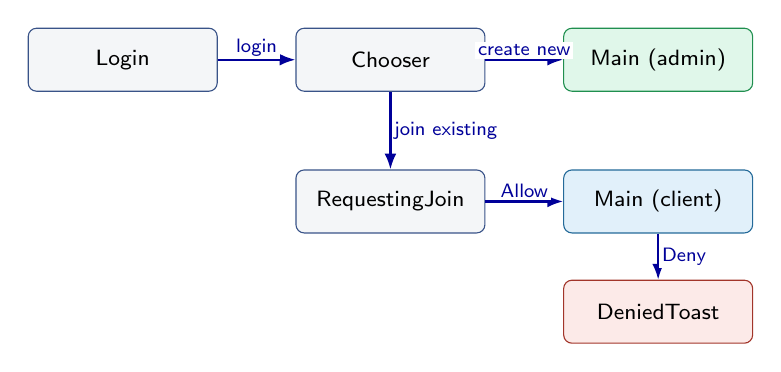
\begin{tikzpicture}[
  every node/.style={font=\sffamily\footnotesize},
  state/.style={
    draw=nixblue!70!black, fill=soft, rounded corners=3pt,
    minimum width=2.4cm, minimum height=0.8cm, align=center,
    inner sep=3pt,
  },
  admin/.style={
    draw=admitted!70!black, fill=admitted!15, rounded corners=3pt,
    minimum width=2.4cm, minimum height=0.8cm, align=center,
    inner sep=3pt,
  },
  client/.style={
    draw=peer!70!black, fill=peer!15, rounded corners=3pt,
    minimum width=2.4cm, minimum height=0.8cm, align=center,
    inner sep=3pt,
  },
  terminal/.style={
    draw=router!70!black, fill=router!12, rounded corners=3pt,
    minimum width=2.4cm, minimum height=0.8cm, align=center,
    inner sep=3pt,
  },
  trans/.style={-{Latex[length=2mm]}, thick, blue!60!black},
  trlbl/.style={font=\scriptsize\sffamily, fill=white, inner sep=1pt, midway},
]
  % Top row: admin path
  \node[state]   (login)   at (0, 0)   {Login};
  \node[state]   (chooser) at (3.4, 0) {Chooser};
  \node[admin]   (mainAd)  at (6.8, 0) {Main (admin)};

  % Bottom row: client path
  \node[state]    (req)    at (3.4, -1.8) {RequestingJoin};
  \node[client]   (mainCl) at (6.8, -1.8) {Main (client)};
  \node[terminal] (denied) at (6.8, -3.2) {DeniedToast};

  \draw[trans] (login)        -- node[trlbl,above]{login} (chooser);
  \draw[trans] (chooser)      -- node[trlbl,above]{create new}    (mainAd);
  \draw[trans] (chooser.south) -- node[trlbl,right]{join existing} (req.north);
  \draw[trans] (req)          -- node[trlbl,above]{Allow}         (mainCl);
  \draw[trans] (mainCl.south) -- node[trlbl,right]{Deny}          (denied.north);
\end{tikzpicture}
\caption{Launcher screens and main transitions. Green denotes the
admin role; blue denotes the client role. From every non-Login
state, \texttt{logout} returns to Login. From the client's main
screen, \texttt{pick\_session} returns to the chooser; this is
the mid-run swap mediated by \texttt{config\_changed} (see
Section~\ref{sec:howRouterUses}).}
\label{fig:launcher-fsm}
\end{figure}

Each transition arrow corresponds to one Tauri command, and each
command is a wrapper around one or two framework calls. The
state machine is therefore the framework's behaviour as exposed
to the user.

% ==============================================================
\section{What the Framework Does Not Do}
% ==============================================================

The framework deliberately excludes several adjacent concerns.

\subsection{Operational policy}
The framework does not decide which CNs to admit or deny; it only
provides the cryptographic primitives needed to act on a
decision. The decision is made by the admin operator through the
user interface.

\subsection{Identity beyond the certificate CN}
An operator is identified by the CN in the leaf certificate.
Mapping a CN to a person (a name, an email address, a team) is
out of scope. A future requirement for human-readable identity
would be implemented in the launcher, not in the framework.

\subsection{Agent business logic}
The demo agents (\texttt{ping} and \texttt{pong}) consist of a
small amount of integration code around the framework. Real
agents are expected to implement additional behaviour (such as
inference, sensor fusion, or scheduling). The framework does not
own that logic. The guarantee provided by the framework is that
the bytes an agent passes to \texttt{cipher.encrypt} are
delivered intact to every admitted peer's \texttt{cipher.decrypt}.

\subsection{Persistence across restarts}
\texttt{DverseConfig} is held in memory and is not persisted.
Restarting any binary that uses the framework returns it to a
clean state. This is intentional for the operator-facing case;
login is required to be explicit. Agents re-acquire their
certificates on each launch when needed, and the short-lived
leaf certificates can be re-issued against the same Keycloak
token.

% ==============================================================
\section{Tying It Back to the Project}
% ==============================================================

The design challenge of the semester is a decentralised
communication platform for humans and AI agents.
\texttt{bot\_framework} is the foundation on which the rest of
the project's deliverables are built. The security pivot
described in the sibling document is implemented in
\texttt{session\_crypto.rs} and \texttt{payload\_crypto.rs}; the
live agent graph in the launcher consumes the heartbeats from
\texttt{AgentAnnouncer}; the demo agents are the smallest
programs that exercise the framework end to end. A reader who
has finished this document should be able to open any file in
the DVerse repository and identify the part of the framework on
which the file relies.

% ==============================================================
\section*{Glossary}
\addcontentsline{toc}{section}{Glossary}
% ==============================================================

\begin{description}[leftmargin=2.4cm, style=nextline, font=\sffamily\bfseries]
  \item[admission] The handshake by which a candidate node
        becomes a member of a session and obtains the
        session's Megolm \texttt{SessionKey}.
  \item[A record] DNS resource record mapping a hostname to
        an IPv4 address; published by mDNS responders for the
        \texttt{.local} hostname.
  \item[bot\_framework] The Rust crate at
        \path{src/bot_framework/} that consolidates the
        platform's mTLS, admission, and payload-encryption
        primitives.
  \item[CN] Common Name. The subject field of a TLS
        certificate, used in this project as the operator's
        identifier on the fabric.
  \item[\texttt{config\_changed}] A \texttt{tokio::sync::Notify}
        on the router state. The launcher rings it after
        staging a new \texttt{DverseConfig} to force the
        router to swap roles.
  \item[crate] A Rust compilation unit. The DVerse workspace
        contains five crates; \texttt{bot\_framework} is one
        of them.
  \item[Curve25519] An elliptic-curve key-exchange primitive
        used by Olm; the framework binds the operator's
        Curve25519 identity key to the TLS certificate via a
        separate ECDSA signature.
  \item[DverseConfig] The struct that holds the operator's
        runtime configuration: router endpoint, certificate
        directory, session role and identifier, and OIDC
        credentials.
  \item[ECDSA] Elliptic Curve Digital Signature Algorithm. The
        signature scheme used for both the TLS leaf
        certificate and the identity-binding signature.
  \item[fabric] The set of mutually authenticated Zenoh peers
        connected through the same mTLS-protected mesh.
  \item[GroupReceiver] The Megolm decrypt half. One per known
        peer in the cipher's \texttt{receivers} map.
  \item[GroupSender] The Megolm encrypt half. One per
        process. Each \texttt{GroupSender} produces messages
        tagged with a unique \texttt{session\_id}.
  \item[Keycloak] An open-source identity-and-access
        management product. In DVerse, it is the OIDC provider
        against which Step-CA authenticates.
  \item[mDNS] Multicast DNS (RFC 6762). Link-local hostname
        resolution on UDP port 5353; the DVerse V3
        implementation uses the Rust \texttt{mdns-sd} crate
        rather than the system-level Avahi daemon.
  \item[Megolm] A group-ratchet cryptographic primitive from
        the Matrix project, used by DVerse to encrypt every
        agent payload.
  \item[mTLS] Mutual Transport Layer Security, in which both
        ends of a TLS connection authenticate with
        certificates.
  \item[OIDC] OpenID Connect, the identity layer on top of
        OAuth 2.0 that Keycloak implements and that Step-CA
        consumes to validate enrolment tokens.
  \item[Olm] A one-to-one cryptographic ratchet from the
        Matrix project, used by DVerse to wrap the Megolm
        session key for a specific requester at admission
        time.
  \item[\texttt{PayloadCipher}] The framework's per-process
        encryption type: one \texttt{GroupSender} and a map
        of \texttt{GroupReceiver}s keyed by peer
        \texttt{session\_id}.
  \item[prekey] A short-lived Curve25519 key published by the
        admission requester. Consumed once by the admin's Olm
        session at admission time and discarded.
  \item[\texttt{session\_id}] The Megolm identifier of a
        \texttt{GroupSender}; receivers are indexed by the
        sender's identifier so that decryption can dispatch
        by the wire envelope.
  \item[\texttt{SessionKey}] The Megolm key material
        exchanged during admission and installed by the
        requester as a \texttt{GroupReceiver}.
  \item[Step-CA] An online certificate authority (Smallstep)
        configured with an OIDC provisioner that
        authenticates against Keycloak.
  \item[Tauri] A Rust framework for building desktop
        applications with a web-based frontend. The DVerse
        launcher uses Tauri 2.
  \item[tokio] The asynchronous runtime used by the DVerse
        Rust code; provides the \texttt{Notify} primitive
        behind \texttt{config\_changed}, the task spawner used
        by the relay, and the I/O reactor used by Zenoh.
  \item[vodozemac] A Rust implementation of the Matrix Olm
        and Megolm cryptographic protocols.
  \item[Zenoh] A decentralised pub/sub and query messaging
        protocol from the Eclipse Foundation. The DVerse data
        plane is built on Zenoh sessions.
\end{description}

% ==============================================================
\bibliographystyle{plainnat}
\bibliography{\jobname}

\end{document}
